
\chapter{Apéndice}
\label{cap:manual}


\section{Registro y levantamiento de información}

\begin{figure}[H]
\centering
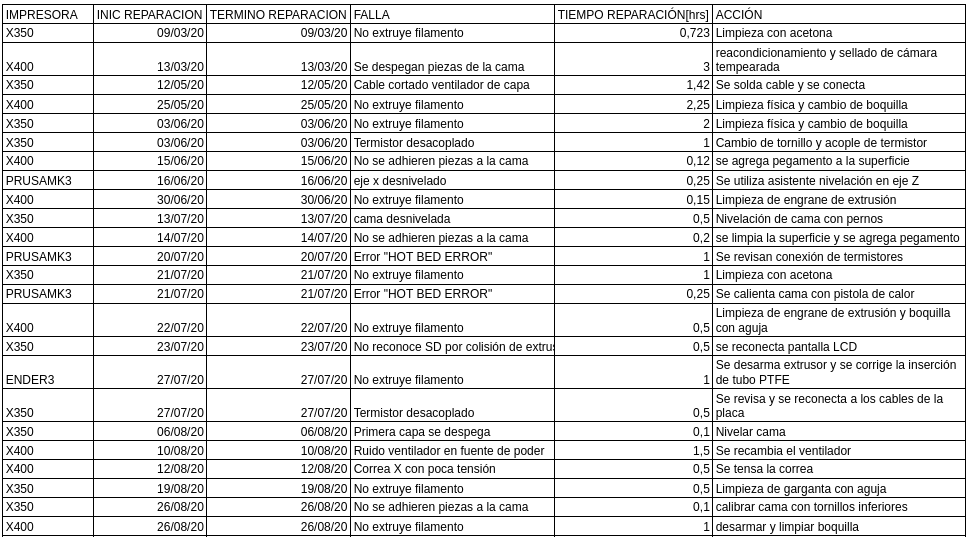
\includegraphics[scale=0.6]{images/registrofallas1.png}
\caption{Registro de fallas en taller de impresión 3D.}
\label{registrofallas1}
\end{figure}

\begin{figure}[H]
\centering
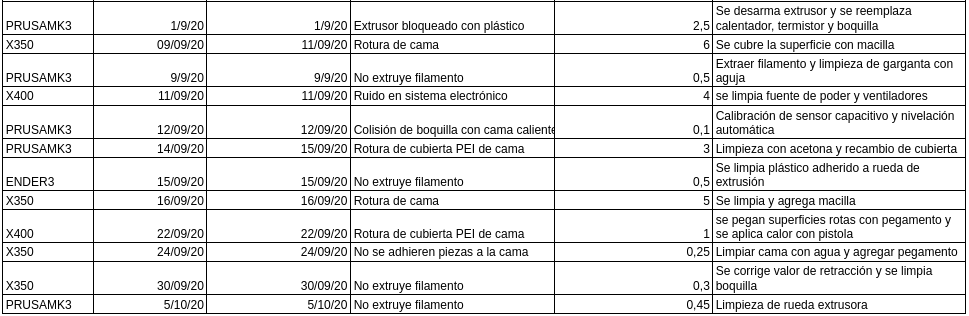
\includegraphics[scale=0.6]{images/registrofallas2.png}
\caption{Continuación de registros de fallas en taller de impresión 3D.}
\label{registrofallas2}
\end{figure}



\section{Análisis de Weibull}

\begin{figure}[H]
\centering
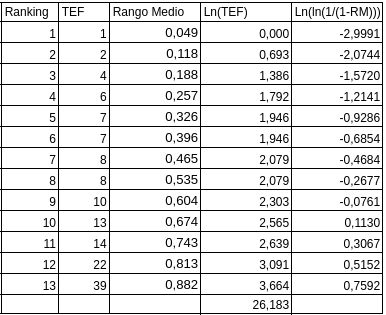
\includegraphics[scale=0.8]{images/linweibx350.png}
\caption{Tiempo entre fallas, rango medio y linealización de función para análisis de Weibull para impresora X350.}
\label{linweibx350}
\end{figure}


\begin{figure}[H]
\centering
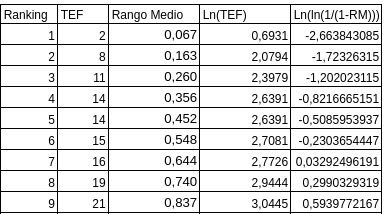
\includegraphics[scale=0.8]{images/linweibx400.png}
\caption{Tiempo entre fallas, rango medio y linealización de función para análisis de Weibull para impresora X400.}
\label{linweibx400}
\end{figure}


\begin{figure}[H]
\centering
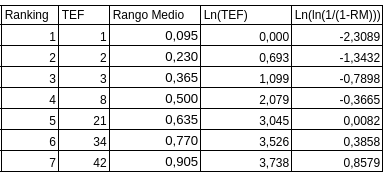
\includegraphics[scale=0.8]{images/linweibmk2.png}
\caption{Tiempo entre fallas, rango medio y linealización de función para análisis de Weibull para impresora Prusa MK2.}
\label{linweibmk2}
\end{figure}



\begin{figure}[H]
\centering
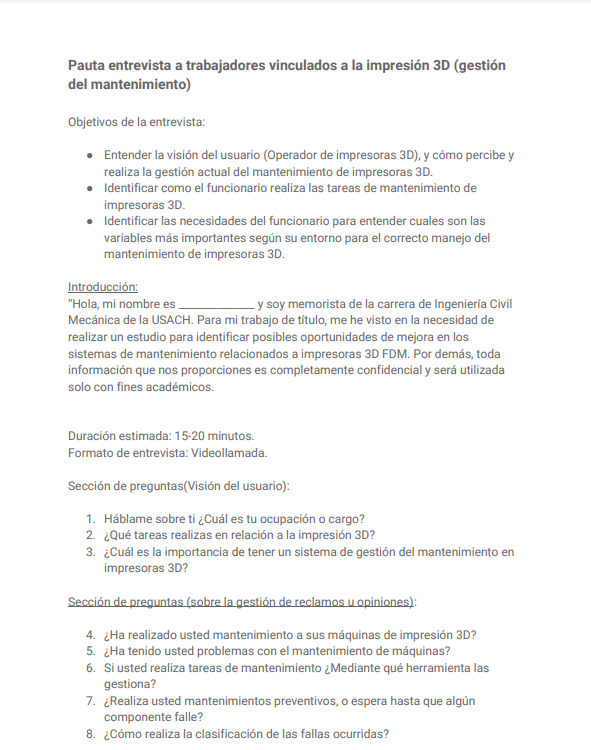
\includegraphics[scale=1]{images/pauta1.png}
\caption{Pauta de preguntas para entrevista personal.}

\end{figure}

\begin{figure}[H]
\centering
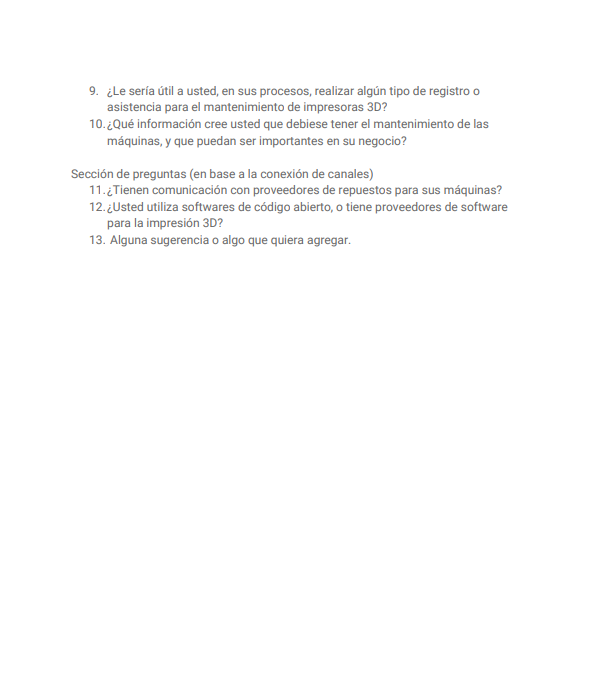
\includegraphics[scale=1]{images/pauta2.png}
\caption{Continuación de pauta de preguntas para entrevista personal}

\end{figure}

\begin{figure}[H]
\centering
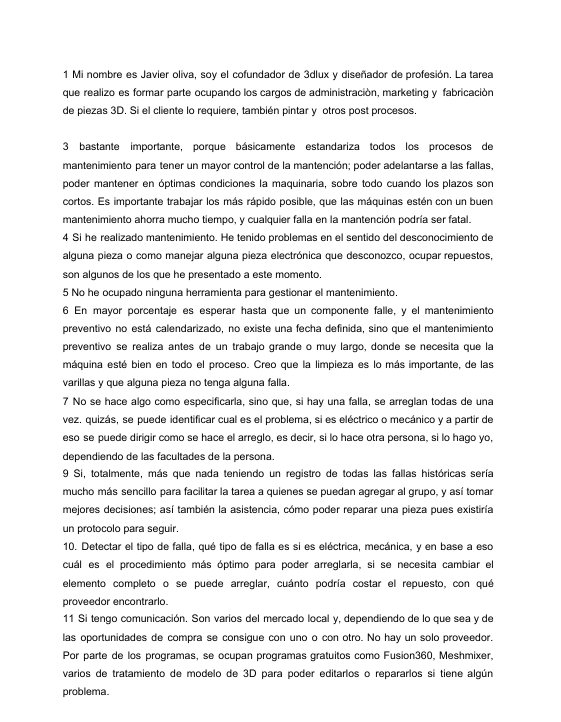
\includegraphics[scale=1]{images/resp1.png}
\caption{Respuestas de entrevista personal}

\end{figure}

\begin{figure}[H]
\centering

\includegraphics[scale=1]{images/resp2.png}
\caption{Continuación de respuestas de entrevista personal.}

\end{figure}